This chapter details the controller design of the model based controller. The performance of the controller is tested with the aid of a simulation model. The model as derived in Chapter \ref{chap2} will be used with the parameters found in Chapter \ref{chap3}. In order for the model to be complete pump dynamics should be added. These pumps have a major influence on the dynamics of the system. Once these are determined the Jacobian controller can be implemented on the dynamic model. 


\section{Jacobian control}


The controller designed in this study includes jacobian information. Jacobian control is a widely used type of model-based controller for positioning classic robots. As mentioned in Chapter \ref{chapter1}, jacobian controllers only use model information on velocity and position level. Thus, system dynamics are not used in this control law.


The Jacobian controller proposed is an adapted version of the one presented in \cite{MOOSAVIAN20071226}. This work shows that a computed torque controller can be approximated by a more straightforward control law involving the Jacobian transpose. This approximation holds if high enough control gains are used. This work only uses a proportional and derivative action to reduce the error. In order to remove the steady-state error, an integrator gain is added this controller. This Jacobian transposed control law is given by,


\begin{equation}
    \tau_{set} = \begin{bmatrix}J(\sigma,t)\end{bmatrix}^\top \Big(K_p e + K_i \int_0^t e \hspace{2pt} ds +  K_d \dot{e}\Big), 
    \label{eq:tau}
\end{equation}

where $\tau_{set} \in \mathbb{R}^2$ is the control input vector with control input moment and force. The Jacobian is determined with equation \ref{eq2:J}. Furthermore, $K_p,K_i $ and $K_d \in \mathbb{R}^{2\times 2}$ are diagonal gain matrices. Here $K_p$ penalizes proportional to the error, $K_i$ contributes to the sum of the error over time, and $K_d$ penalized the error derivative. The error $e \in \mathbb{R}^2$ is defined as the difference between reference position and the actual position in the (x,y)-plane. Therefore not the entire Jacobian of dimension $6 \times 2$, but only the entries mapping modal coordinate velocity to linear velocity in x-y plane. As mentioned this Jacobian is space-time variant. Therefore, in the control law this Jacobian is calculated real-time based on the actual kinematic configuration of the actuator. 

The actual system does not allow to induce forces and moments directly. Therefore this control input should be mapped to pressure. Here the mapping as found with finite element analysis in Chapter \ref{chap3} is used to map pressure to force. Based on the desired control input, a reference pressure can be formulated as,

\begin{equation}
    p_{ref} = H^{-1}\tau,
\end{equation}


where $p_{ref} \in \mathbb{R}^2$ is the reference pressure for each bellow. In order for this reference pressure to be reached a second controller is necessary. This low-level controller is used to set the input voltage that is supplied to the pumps.  The volt input is regulated via pulse width modulation (pwm). Since the Raspberry PI is equipped with a 12bit ADC (analog-digital converter), it is possible calculate the pwm input as, $\textit{pwm} = \frac{2^{12} V}{V_{max}} $, where $V_{max}$ is equal to 12 volt. This control law is given by,


\begin{equation}
    pwm_{set} = K_{pp}e_p \hspace{10pt} \text{with} \hspace{10pt} e_p = p_{ref} - p,
\end{equation}



where $pwm_{set}$ is the input voltage and $K_{pp} \in \mathbb{R}^{2\times 2}$ a diagonal gain matrix. Furthermore, $e_p$ is the pressure error, which is the difference between reference pressure and actual pressure. Observe that only a proportional action is used. The integral action of the jacobian controller will already ensure no steady-state error. 




\section{Pump Dynamics}





Besides soft robot actuator properties also the actuator properties are involved. To this end the pump dynamics are determined. In the proposed control architecture, the Jacobian controller is accompanied by a pressure controller. To this end, the pump dynamics need to be determined. Initially, we determine the pump dynamics by  connecting the pump directly to the pressure sensor. This yielded poor performance once connected to the soft actuator. To suppress noise levels and capture the actual system dynamics better the set-up is slightly adapted. Furthermore we make the following assumption:


\begin{theorem}
Both air pumps have the equal pump characteristics, therefore the system dynamics of a single air pump need to be determined.
\end{theorem}


To determine the pump dynamics the pump is connected directly to the pressure sensor using a short flexible silicone hose. The pump is powered by an electric 12V DC motor, and uses membranes to create pressure. The pump characteristics are obtained by observing the systems response for various volt step inputs between 1 and 6 Volt. Although the pumps are able to operate at 12 Volt, only a maximum step input of 6V is possible for this set-up. The pressure sensor measures absolute pressures between 0 and 25 PSI, which is equivalent to a maximum of 172 kPa. Depending on weather conditions, the maximum theoretically measurable pressure is around 72 kPa. However, experiments have shown results up to 80 kPa are possible. The resulting step responses are shown in Figure (\ref{fig1:pump_dynamcis}).

\begin{figure}[H]
    \centering
    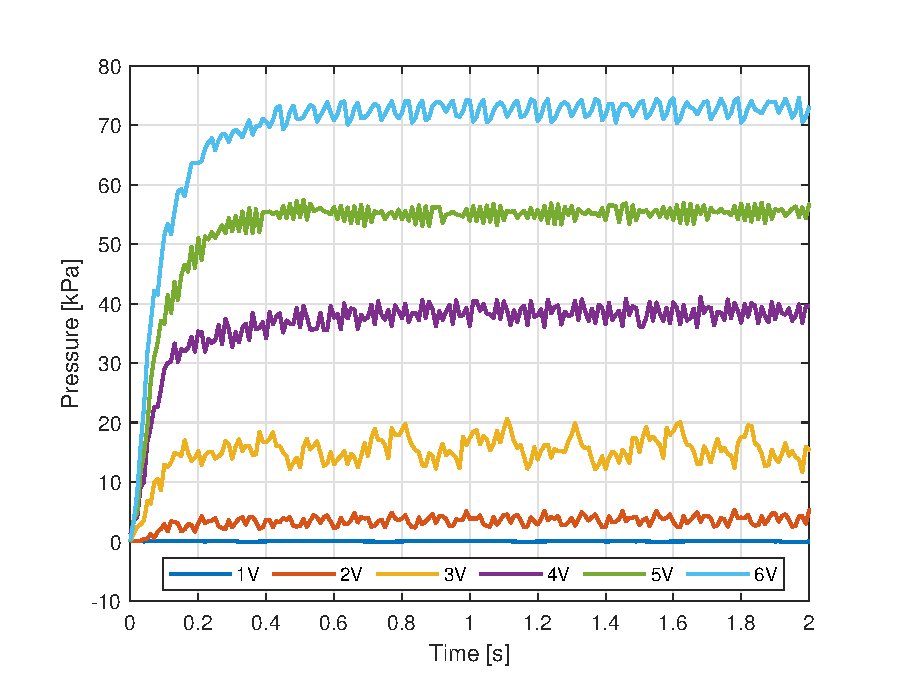
\includegraphics[width = 0.6\textwidth]{Figures/Chapter3/stepresponsdirect16V.eps}
    \caption{Step response for volt step input between 1V and 6V.}
    \label{fig1:pump_dynamcis}
\end{figure}

Multiple observations can be made based on the step response of Figure (\ref{fig1:pump_dynamcis}). A first glance reveals first order system behaviour as  pressure increase seems to be proportional to the actual pressure. However, the steady-state pressure is not proportional to the input volt for all step responses. The reason for this behaviour is thought to be friction. For 1 and 2 volt input static friction dominates, resulting in no to very small pressure increase. At 3 volt the transition between dry and kinetic friction is observed. The first order system characteristic become better visible, although the pressure response is chattering. Furthermore, we see a rise time of comparable order for step inputs of 4V and above. After around 0.5 seconds the steady-state pressure is reached. For all step inputs oscillations are observed around the steady-state pressure. This phenomena is caused by the fact that there is almost no passive leakage from the small control volume. When the pump valves open and air is pressed into the system the air waves are created. For the step input of 5 volt the valve dynamics can be clearly seen, as the dense green spikes.

An improved pump model can be obtained by altering the set-up. To this end, the actuator and an air vessel are connected to the system. Previous research showed that adding an air vessel will reduce oscillatory behaviour, at the cost of bandwidth \cite{proper}. The air vessel will increase the control volume of the entire system. When the valves open and additional air is pressed in the system, the relative pressure change is smaller. Additionally, when the actuator expands the relative volume increase will also be smaller. This will cause the system to respond slower to a step input. Furthermore, the maximum achievable pressure is lower. The addition of air vessel and actuator will increase the passive leakage of the system.

For the adapted system the step response is determined for volt steps between 2 and 12 volt. The results are shown in Figure \ref{fig3:pump_dynamics_adapted}.

\begin{figure}[H]
    \centering
    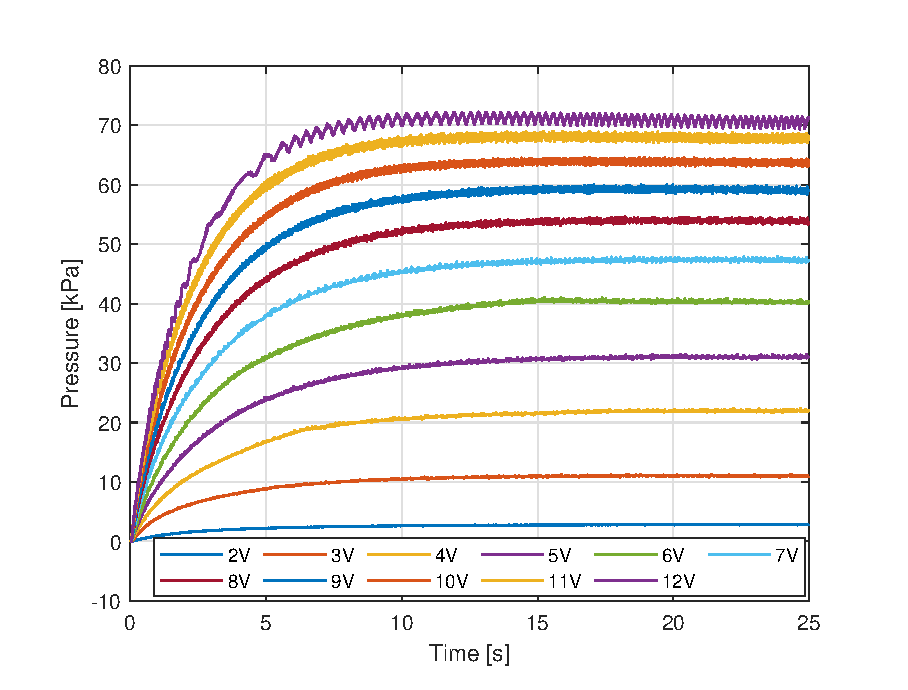
\includegraphics[width = 0.6\textwidth]{Figures/Chapter3/step212V.eps}
    \caption{Step response for volt step input between 2V and 12V for the system including air vessel and actuator.}
    \label{fig3:pump_dynamics_adapted}
\end{figure}


Based on the step responses of Figure (\ref{fig3:pump_dynamics_adapted}) we try to capture the pump dynamics in a model. The time response of a first order linear system responding to a step input is given by, 

\begin{equation}
    p(t,V) = K(1-e^{-t/\tau})V,
    \label{eq3:firstordermodel}
\end{equation}

where $p$ is the pressure at time $t$ in kPa. DC-gain $K$ [kPa/V] determines the maximum pressure, time constant $\tau_s$ [1/s] determines the growth rate of the exponential function. Furthermore, $V$ is the input volt. 

An attempt to fit the linear first order model of (\ref{eq3:firstordermodel}) did not result in an accurate description of the pump dynamics for all step inputs. Therefore an alternative description of the pump dynamics is proposed. In this description DC-gain $K$ is replaced by a nonlinear function $K(V)$. Additionally, a linear function $\tau_s(V)$ is proposed. This adaption makes the original model non-linear. Additionally, we are aware that by introducing these functions the terminology time `constant' is used incorrectly.


Based on (\ref{eq3:firstordermodel}) an indication of the gradient between constant $K$ and $V$ can be estimated. The DC-gain can be found by dividing the steady-state pressure by its corresponding volt input. The steady-state pressure for each step input is estimated by taken the mean over the last 10 seconds of data. A similar approach is done for determining time constant $\tau_s$. For a first order system it can be proven that this time constant is equal to time at which 63\% of the steady state value is reached. The corresponding relations for $K(V)$ and $\tau_s(V)$ are shown in Figure \ref{fig3:Kest} and Figure \ref{fig3:tauest}, respectively.
\newpage

\begin{figure}[H]
\begin{minipage}[b]{0.48\linewidth}
\centering
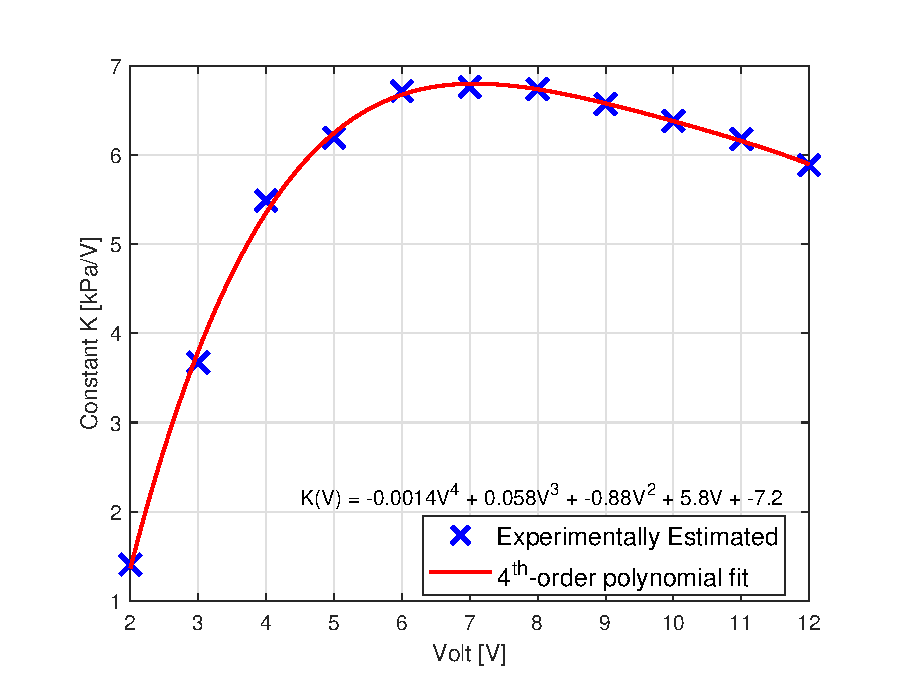
\includegraphics[width=\textwidth]{Figures/Chapter3/Kest.eps}
\caption{Experimental estimate of `constant' $K$ and fourth order fit.}
\label{fig3:Kest}
\end{minipage}
\begin{minipage}[b]{0.48\linewidth}
\centering
\includegraphics[width=\textwidth]{Figures/Chapter3/tauest.eps}
\caption{Experimental estimate of time `constant' $\tau$ and linear fit.}
\label{fig3:tauest}
\end{minipage}
\end{figure}

Figure \ref{fig3:Kest} shows a fourth-order polynomial fit through DC-gain $K$. For step inputs larger than 8 volt the DC-gain drops. This indicates that the air pump is less efficient for these volt inputs. This could be caused an increased temperature of the air pump. Another explanation for this behaviour is an increased passive leakage of the system, as steady-state pressure is higher for high volt inputs. Up till 5V the pumps do not adhere to what is expected. The DC-gains found in this region indicate inefficient pump behaviour. It is believed that this is caused by friction.

Figure \ref{fig3:tauest} shows the estimated time constants, with a linear fit. Clearly the estimated time constant for 2 and 3 volt do not follow this linear trend line. Therefore, this data point where excluded from the linear fit. A possible explanation for these outliers is the friction acting at these voltage inputs, and are therefore not reliable. Furthermore, we see the time constant decreasing for a increasing volt. This means that the pump has a faster response for higher volt input. This can make sense as the total power supplied to the air pumps is higher. 


The obtained measurement fits for $K$ and $\tau_s$ can be substituted in (\ref{eq3:firstordermodel}) resulting in an expression as,

\begin{equation}
    p(t,V) = K(V)(1-e^{-t/\tau_s(V)})V.
    \label{eq3:firstodernonlinearmodel}
    \end{equation}

The derived first order model of (\ref{eq3:firstodernonlinearmodel}) can be plotted against the experimental results of Figure (\ref{fig3:pump_dynamics_adapted}), this is shown in Figure (\ref{fig3:expvsfitpres}).

\newpage

\begin{figure}[H]
    \centering
    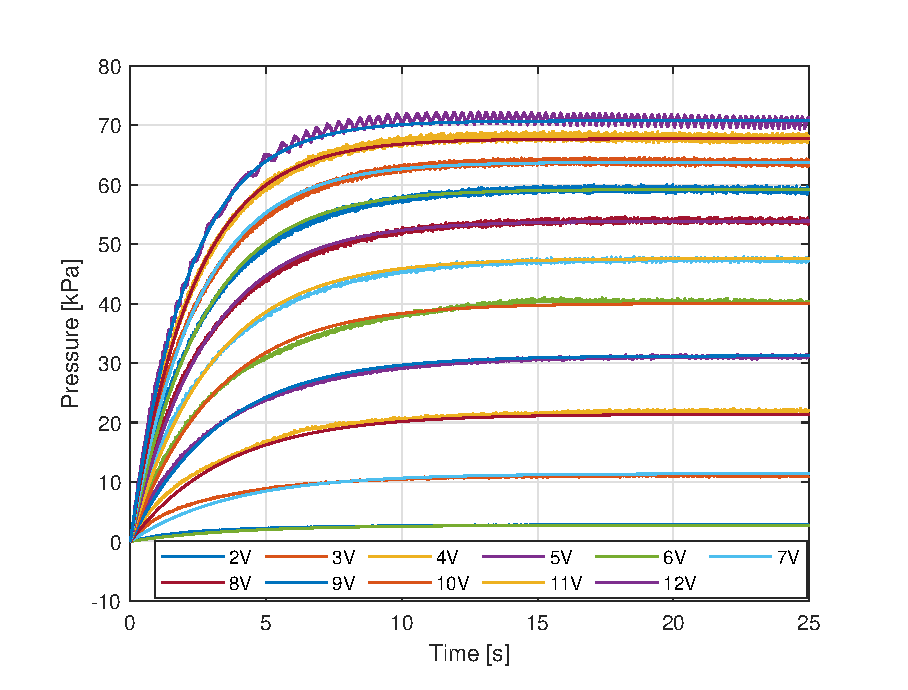
\includegraphics[width = 0.7\textwidth]{Figures/Chapter3/expfit.eps}
    \caption{Experimental results and the derived nonlinear pressure model.}
    \label{fig3:expvsfitpres}
\end{figure}

Above figure shows that the derived model captures the behaviour of the system with actuator and air vessel accurately. The steady-state pressure is close to the experimental value for all volt step inputs. As expected, the rise time for the 1 and 2 volt step inputs are not captured that well by this model.

The obtained dynamic response is arguable from a physical point of view. The dynamic model for the air pumps is fit to a first order linear system by introducing non-linearity's. Therefore the obtained model is very specific and does not allow for a change in parameters. Therefore this model can not be used in a changed set-up. Furthermore it should be noted that the fourth order fit used to describe the DC-gain is found negative for Volt input equal to 0. From a physical perspective this is not possible. At 0 volt input, the DC-gain should be equal to 0. Therefore the model is only deemed valid in the volt input range where $K$ is positive.

\hl{in this section sinusoidal response of the pump model should be added for experimental verification}


\section{Controller in Simulation}

The dynamical model that was derived in Chapter \ref{chap2} can be used to test the applicability of the Jacobian controller. Recall the dynamic model as, 


\begin{equation}
    M(q)\Ddot{q} + D\dot{q} + K(q)q = \tau \hspace{10pt} \text{with} \hspace{10pt} \tau = Hp.
    \label{eq4:dynamicmodel}
\end{equation}

The parameter identification allows to obtain the entries of mass matrix $M$ and stiffness matrix $K$. With the determined stiffness' matrix $K = \text{diag}([K_\kappa \hspace{3pt} K_\epsilon])$. The diagonal damping matrix is equal is represented by $D = \text{diag}([D_\kappa \hspace{3pt} D_\epsilon])$. Damping properties have not been determined experimentally, as the actuator cannot be actuated such that a measurable free excitation is induced in a single axis. Therefore the damping parameters are chosen iteratively. In Appendix \ref{app4}, a free oscillation of the dynamic model is presented. Here the effect of damping on the systems response is further elucidated. Furthermore an analysis on the accuracy of the model is provided.

The dynamic model of (\ref{eq4:dynamicmodel}) allows for numeric solving by reformulating the model to a second order state-space formulation as,

\begin{equation}
     \begin{bmatrix} \dot{x}  \end{bmatrix}   = \underbrace{  \begin{bmatrix} O_2 & I_2 \\ -M(q)^{-1}K(q)  & -M(q)^{-1} D \end{bmatrix}   }_{A} \begin{bmatrix} x \end{bmatrix}  +      \underbrace{\begin{bmatrix} O_2 \\ M(q)^{-1}H   \end{bmatrix}   }_{B}    \begin{bmatrix} p_1\\ p_2  
     \end{bmatrix}, 
     \label{eq4:SS}
\end{equation}

with state vector $x = \begin{bmatrix} \kappa \hspace{3pt} \epsilon \hspace{3pt} \dot{\kappa}  \hspace{3pt} \dot{\epsilon}  \end{bmatrix}^{\top}$. Here matrix $A \in \mathbb{R}^{4\times 4}$ contains all elements with respect to the system dynamics. Matrix $B\in\mathbb{R}^{4 \times 2}$ is the control input vector. Mind the substitution of the mapping matrix, hence control input is pressure instead of force and moment. 

Above state-space does not allow to give an accurate system description as the pump dynamics are not included in this representation. Therefore an adapted state space formulation is presented as,

\begin{equation}
     \begin{bmatrix} \dot{x}  \end{bmatrix}   =   \underbrace{ \begin{bmatrix} O_2 & I_2 & O_2 \\ -M(q)^{-1}K(q)  & -M(q)^{-1} D & O_2 \\
     O_2 & O_2    & -\frac{1}{\tau_s(V)}I_2\ \end{bmatrix}   }_A   \begin{bmatrix} x \end{bmatrix}  + \underbrace{      \begin{bmatrix} O_2 & O_2 \\ M(q)^{-1}H & O_2 \\ O_2 & \frac{K(V)}{\tau_s(V)} I_2 \end{bmatrix} }_B      \begin{bmatrix} p_1 \\ p_2  \\ V_1 \\ V_2 \end{bmatrix},
     \label{eq:ssp}
\end{equation}


where state vector $x$ is extended to $x = [\kappa \hspace{3pt} \epsilon \hspace{3pt} \dot{\kappa} \hspace{3pt} \dot{\epsilon} \hspace{3pt} p_1 \hspace{3pt} p_2]$. Here matrix $A \in \mathbb{R}^{6\times 6}$ containing the dynamics is extended. Additionally input matrix $B \in \mathbb{R}^{6\times 4}$ is extended to allow volt input. In this simulation model, the volt input is limited to be between 0 and 12 volt. This constrains the system such that negative pressures can not be used to control the system. 

Above state space model and presented Jacobian controller is implemented in \MATLAB. Figure  shows a simulation o







\hl{check script, something goes wrong no positive pressures}